% Created by tikzDevice version 0.10.1 on 2018-03-03 10:35:26
% !TEX encoding = UTF-8 Unicode
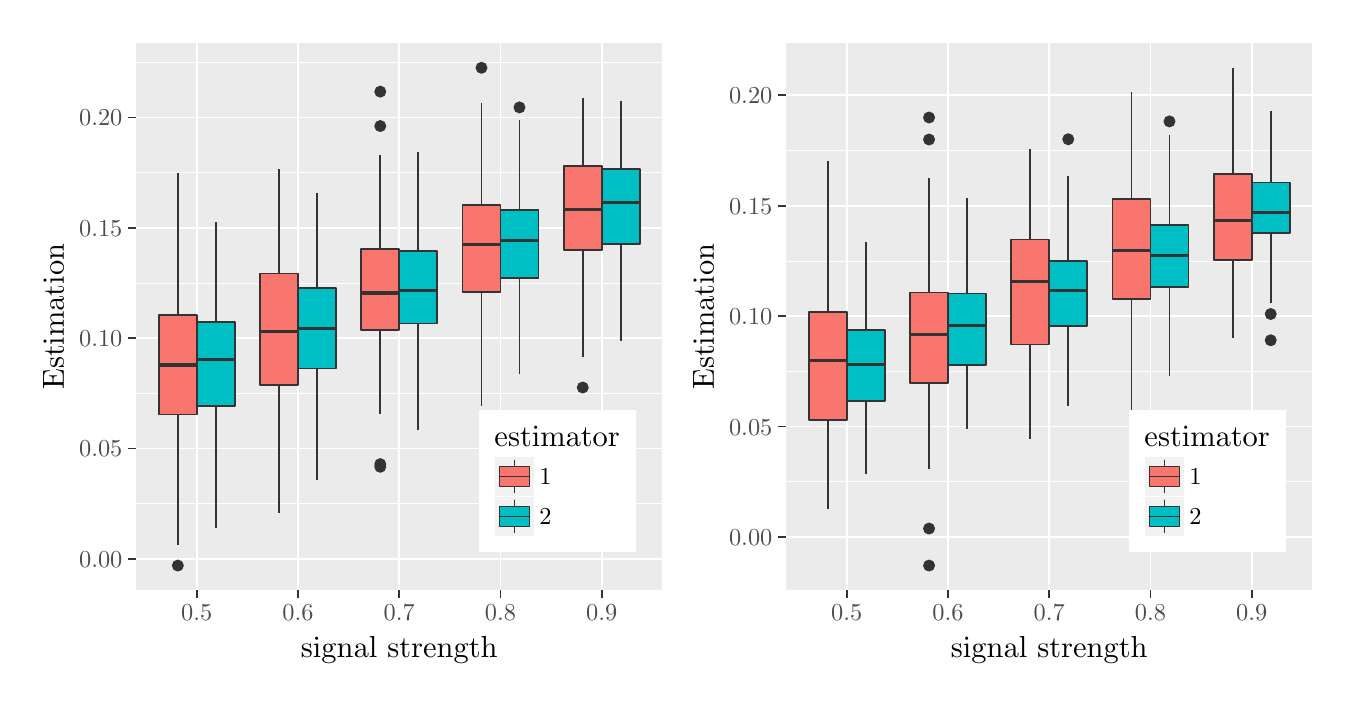
\begin{tikzpicture}[x=1pt,y=1pt]
\definecolor{fillColor}{RGB}{255,255,255}
\path[use as bounding box,fill=fillColor,fill opacity=0.00] (0,0) rectangle (469.76,234.88);
\begin{scope}
\path[clip] (  0.00,  0.00) rectangle (234.88,234.88);
\definecolor{drawColor}{RGB}{255,255,255}
\definecolor{fillColor}{RGB}{255,255,255}

\path[draw=drawColor,line width= 0.6pt,line join=round,line cap=round,fill=fillColor] (  0.00,  0.00) rectangle (234.88,234.88);
\end{scope}
\begin{scope}
\path[clip] ( 39.17, 31.53) rectangle (229.38,229.38);
\definecolor{fillColor}{gray}{0.92}

\path[fill=fillColor] ( 39.17, 31.53) rectangle (229.38,229.38);
\definecolor{drawColor}{RGB}{255,255,255}

\path[draw=drawColor,line width= 0.3pt,line join=round] ( 39.17, 62.88) --
	(229.38, 62.88);

\path[draw=drawColor,line width= 0.3pt,line join=round] ( 39.17,102.76) --
	(229.38,102.76);

\path[draw=drawColor,line width= 0.3pt,line join=round] ( 39.17,142.64) --
	(229.38,142.64);

\path[draw=drawColor,line width= 0.3pt,line join=round] ( 39.17,182.53) --
	(229.38,182.53);

\path[draw=drawColor,line width= 0.3pt,line join=round] ( 39.17,222.41) --
	(229.38,222.41);

\path[draw=drawColor,line width= 0.6pt,line join=round] ( 39.17, 42.94) --
	(229.38, 42.94);

\path[draw=drawColor,line width= 0.6pt,line join=round] ( 39.17, 82.82) --
	(229.38, 82.82);

\path[draw=drawColor,line width= 0.6pt,line join=round] ( 39.17,122.70) --
	(229.38,122.70);

\path[draw=drawColor,line width= 0.6pt,line join=round] ( 39.17,162.59) --
	(229.38,162.59);

\path[draw=drawColor,line width= 0.6pt,line join=round] ( 39.17,202.47) --
	(229.38,202.47);

\path[draw=drawColor,line width= 0.6pt,line join=round] ( 61.11, 31.53) --
	( 61.11,229.38);

\path[draw=drawColor,line width= 0.6pt,line join=round] ( 97.69, 31.53) --
	( 97.69,229.38);

\path[draw=drawColor,line width= 0.6pt,line join=round] (134.27, 31.53) --
	(134.27,229.38);

\path[draw=drawColor,line width= 0.6pt,line join=round] (170.85, 31.53) --
	(170.85,229.38);

\path[draw=drawColor,line width= 0.6pt,line join=round] (207.43, 31.53) --
	(207.43,229.38);
\definecolor{drawColor}{gray}{0.20}
\definecolor{fillColor}{gray}{0.20}

\path[draw=drawColor,line width= 0.4pt,line join=round,line cap=round,fill=fillColor] ( 54.26, 40.52) circle (  1.96);

\path[draw=drawColor,line width= 0.6pt,line join=round] ( 54.26,130.94) -- ( 54.26,182.48);

\path[draw=drawColor,line width= 0.6pt,line join=round] ( 54.26, 95.06) -- ( 54.26, 47.80);
\definecolor{fillColor}{RGB}{248,118,109}

\path[draw=drawColor,line width= 0.6pt,line join=round,line cap=round,fill=fillColor] ( 47.40,130.94) --
	( 47.40, 95.06) --
	( 61.11, 95.06) --
	( 61.11,130.94) --
	( 47.40,130.94) --
	cycle;

\path[draw=drawColor,line width= 1.1pt,line join=round] ( 47.40,112.98) -- ( 61.11,112.98);

\path[draw=drawColor,line width= 0.6pt,line join=round] ( 67.97,128.59) -- ( 67.97,164.64);

\path[draw=drawColor,line width= 0.6pt,line join=round] ( 67.97, 98.15) -- ( 67.97, 54.15);
\definecolor{fillColor}{RGB}{0,191,196}

\path[draw=drawColor,line width= 0.6pt,line join=round,line cap=round,fill=fillColor] ( 61.11,128.59) --
	( 61.11, 98.15) --
	( 74.83, 98.15) --
	( 74.83,128.59) --
	( 61.11,128.59) --
	cycle;

\path[draw=drawColor,line width= 1.1pt,line join=round] ( 61.11,115.09) -- ( 74.83,115.09);

\path[draw=drawColor,line width= 0.6pt,line join=round] ( 90.83,146.08) -- ( 90.83,183.84);

\path[draw=drawColor,line width= 0.6pt,line join=round] ( 90.83,105.65) -- ( 90.83, 59.48);
\definecolor{fillColor}{RGB}{248,118,109}

\path[draw=drawColor,line width= 0.6pt,line join=round,line cap=round,fill=fillColor] ( 83.98,146.08) --
	( 83.98,105.65) --
	( 97.69,105.65) --
	( 97.69,146.08) --
	( 83.98,146.08) --
	cycle;

\path[draw=drawColor,line width= 1.1pt,line join=round] ( 83.98,124.99) -- ( 97.69,124.99);

\path[draw=drawColor,line width= 0.6pt,line join=round] (104.55,140.75) -- (104.55,175.19);

\path[draw=drawColor,line width= 0.6pt,line join=round] (104.55,111.68) -- (104.55, 71.45);
\definecolor{fillColor}{RGB}{0,191,196}

\path[draw=drawColor,line width= 0.6pt,line join=round,line cap=round,fill=fillColor] ( 97.69,140.75) --
	( 97.69,111.68) --
	(111.41,111.68) --
	(111.41,140.75) --
	( 97.69,140.75) --
	cycle;

\path[draw=drawColor,line width= 1.1pt,line join=round] ( 97.69,126.04) -- (111.41,126.04);
\definecolor{fillColor}{gray}{0.20}

\path[draw=drawColor,line width= 0.4pt,line join=round,line cap=round,fill=fillColor] (127.41,199.33) circle (  1.96);

\path[draw=drawColor,line width= 0.4pt,line join=round,line cap=round,fill=fillColor] (127.41, 76.20) circle (  1.96);

\path[draw=drawColor,line width= 0.4pt,line join=round,line cap=round,fill=fillColor] (127.41,211.76) circle (  1.96);

\path[draw=drawColor,line width= 0.4pt,line join=round,line cap=round,fill=fillColor] (127.41, 77.17) circle (  1.96);

\path[draw=drawColor,line width= 0.6pt,line join=round] (127.41,154.83) -- (127.41,188.78);

\path[draw=drawColor,line width= 0.6pt,line join=round] (127.41,125.72) -- (127.41, 95.33);
\definecolor{fillColor}{RGB}{248,118,109}

\path[draw=drawColor,line width= 0.6pt,line join=round,line cap=round,fill=fillColor] (120.55,154.83) --
	(120.55,125.72) --
	(134.27,125.72) --
	(134.27,154.83) --
	(120.55,154.83) --
	cycle;

\path[draw=drawColor,line width= 1.1pt,line join=round] (120.55,139.00) -- (134.27,139.00);

\path[draw=drawColor,line width= 0.6pt,line join=round] (141.13,154.06) -- (141.13,189.83);

\path[draw=drawColor,line width= 0.6pt,line join=round] (141.13,127.97) -- (141.13, 89.67);
\definecolor{fillColor}{RGB}{0,191,196}

\path[draw=drawColor,line width= 0.6pt,line join=round,line cap=round,fill=fillColor] (134.27,154.06) --
	(134.27,127.97) --
	(147.99,127.97) --
	(147.99,154.06) --
	(134.27,154.06) --
	cycle;

\path[draw=drawColor,line width= 1.1pt,line join=round] (134.27,139.93) -- (147.99,139.93);
\definecolor{fillColor}{gray}{0.20}

\path[draw=drawColor,line width= 0.4pt,line join=round,line cap=round,fill=fillColor] (163.99,220.38) circle (  1.96);

\path[draw=drawColor,line width= 0.6pt,line join=round] (163.99,170.79) -- (163.99,207.56);

\path[draw=drawColor,line width= 0.6pt,line join=round] (163.99,139.46) -- (163.99, 98.25);
\definecolor{fillColor}{RGB}{248,118,109}

\path[draw=drawColor,line width= 0.6pt,line join=round,line cap=round,fill=fillColor] (157.13,170.79) --
	(157.13,139.46) --
	(170.85,139.46) --
	(170.85,170.79) --
	(157.13,170.79) --
	cycle;

\path[draw=drawColor,line width= 1.1pt,line join=round] (157.13,156.53) -- (170.85,156.53);
\definecolor{fillColor}{gray}{0.20}

\path[draw=drawColor,line width= 0.4pt,line join=round,line cap=round,fill=fillColor] (177.71,206.07) circle (  1.96);

\path[draw=drawColor,line width= 0.6pt,line join=round] (177.71,168.88) -- (177.71,201.64);

\path[draw=drawColor,line width= 0.6pt,line join=round] (177.71,144.51) -- (177.71,109.59);
\definecolor{fillColor}{RGB}{0,191,196}

\path[draw=drawColor,line width= 0.6pt,line join=round,line cap=round,fill=fillColor] (170.85,168.88) --
	(170.85,144.51) --
	(184.57,144.51) --
	(184.57,168.88) --
	(170.85,168.88) --
	cycle;

\path[draw=drawColor,line width= 1.1pt,line join=round] (170.85,157.82) -- (184.57,157.82);
\definecolor{fillColor}{gray}{0.20}

\path[draw=drawColor,line width= 0.4pt,line join=round,line cap=round,fill=fillColor] (200.57,104.85) circle (  1.96);

\path[draw=drawColor,line width= 0.6pt,line join=round] (200.57,184.82) -- (200.57,209.49);

\path[draw=drawColor,line width= 0.6pt,line join=round] (200.57,154.64) -- (200.57,115.97);
\definecolor{fillColor}{RGB}{248,118,109}

\path[draw=drawColor,line width= 0.6pt,line join=round,line cap=round,fill=fillColor] (193.71,184.82) --
	(193.71,154.64) --
	(207.43,154.64) --
	(207.43,184.82) --
	(193.71,184.82) --
	cycle;

\path[draw=drawColor,line width= 1.1pt,line join=round] (193.71,169.13) -- (207.43,169.13);

\path[draw=drawColor,line width= 0.6pt,line join=round] (214.29,183.73) -- (214.29,208.38);

\path[draw=drawColor,line width= 0.6pt,line join=round] (214.29,156.72) -- (214.29,121.73);
\definecolor{fillColor}{RGB}{0,191,196}

\path[draw=drawColor,line width= 0.6pt,line join=round,line cap=round,fill=fillColor] (207.43,183.73) --
	(207.43,156.72) --
	(221.15,156.72) --
	(221.15,183.73) --
	(207.43,183.73) --
	cycle;

\path[draw=drawColor,line width= 1.1pt,line join=round] (207.43,171.67) -- (221.15,171.67);
\end{scope}
\begin{scope}
\path[clip] (  0.00,  0.00) rectangle (469.76,234.88);
\definecolor{drawColor}{gray}{0.30}

\node[text=drawColor,anchor=base east,inner sep=0pt, outer sep=0pt, scale=  0.88] at ( 34.22, 39.91) {0.00};

\node[text=drawColor,anchor=base east,inner sep=0pt, outer sep=0pt, scale=  0.88] at ( 34.22, 79.79) {0.05};

\node[text=drawColor,anchor=base east,inner sep=0pt, outer sep=0pt, scale=  0.88] at ( 34.22,119.67) {0.10};

\node[text=drawColor,anchor=base east,inner sep=0pt, outer sep=0pt, scale=  0.88] at ( 34.22,159.55) {0.15};

\node[text=drawColor,anchor=base east,inner sep=0pt, outer sep=0pt, scale=  0.88] at ( 34.22,199.44) {0.20};
\end{scope}
\begin{scope}
\path[clip] (  0.00,  0.00) rectangle (469.76,234.88);
\definecolor{drawColor}{gray}{0.20}

\path[draw=drawColor,line width= 0.6pt,line join=round] ( 36.42, 42.94) --
	( 39.17, 42.94);

\path[draw=drawColor,line width= 0.6pt,line join=round] ( 36.42, 82.82) --
	( 39.17, 82.82);

\path[draw=drawColor,line width= 0.6pt,line join=round] ( 36.42,122.70) --
	( 39.17,122.70);

\path[draw=drawColor,line width= 0.6pt,line join=round] ( 36.42,162.59) --
	( 39.17,162.59);

\path[draw=drawColor,line width= 0.6pt,line join=round] ( 36.42,202.47) --
	( 39.17,202.47);
\end{scope}
\begin{scope}
\path[clip] (  0.00,  0.00) rectangle (469.76,234.88);
\definecolor{drawColor}{gray}{0.20}

\path[draw=drawColor,line width= 0.6pt,line join=round] ( 61.11, 28.78) --
	( 61.11, 31.53);

\path[draw=drawColor,line width= 0.6pt,line join=round] ( 97.69, 28.78) --
	( 97.69, 31.53);

\path[draw=drawColor,line width= 0.6pt,line join=round] (134.27, 28.78) --
	(134.27, 31.53);

\path[draw=drawColor,line width= 0.6pt,line join=round] (170.85, 28.78) --
	(170.85, 31.53);

\path[draw=drawColor,line width= 0.6pt,line join=round] (207.43, 28.78) --
	(207.43, 31.53);
\end{scope}
\begin{scope}
\path[clip] (  0.00,  0.00) rectangle (469.76,234.88);
\definecolor{drawColor}{gray}{0.30}

\node[text=drawColor,anchor=base,inner sep=0pt, outer sep=0pt, scale=  0.88] at ( 61.11, 20.52) {0.5};

\node[text=drawColor,anchor=base,inner sep=0pt, outer sep=0pt, scale=  0.88] at ( 97.69, 20.52) {0.6};

\node[text=drawColor,anchor=base,inner sep=0pt, outer sep=0pt, scale=  0.88] at (134.27, 20.52) {0.7};

\node[text=drawColor,anchor=base,inner sep=0pt, outer sep=0pt, scale=  0.88] at (170.85, 20.52) {0.8};

\node[text=drawColor,anchor=base,inner sep=0pt, outer sep=0pt, scale=  0.88] at (207.43, 20.52) {0.9};
\end{scope}
\begin{scope}
\path[clip] (  0.00,  0.00) rectangle (469.76,234.88);
\definecolor{drawColor}{RGB}{0,0,0}

\node[text=drawColor,anchor=base,inner sep=0pt, outer sep=0pt, scale=  1.10] at (134.27,  7.44) {signal strength};
\end{scope}
\begin{scope}
\path[clip] (  0.00,  0.00) rectangle (469.76,234.88);
\definecolor{drawColor}{RGB}{0,0,0}

\node[text=drawColor,rotate= 90.00,anchor=base,inner sep=0pt, outer sep=0pt, scale=  1.10] at ( 13.08,130.45) {Estimation};
\end{scope}
\begin{scope}
\path[clip] (  0.00,  0.00) rectangle (469.76,234.88);
\definecolor{fillColor}{RGB}{255,255,255}

\path[fill=fillColor] (162.99, 45.36) rectangle (219.68, 96.84);
\end{scope}
\begin{scope}
\path[clip] (  0.00,  0.00) rectangle (469.76,234.88);
\definecolor{drawColor}{RGB}{0,0,0}

\node[text=drawColor,anchor=base west,inner sep=0pt, outer sep=0pt, scale=  1.10] at (168.68, 83.57) {estimator};
\end{scope}
\begin{scope}
\path[clip] (  0.00,  0.00) rectangle (469.76,234.88);
\definecolor{drawColor}{RGB}{255,255,255}
\definecolor{fillColor}{gray}{0.95}

\path[draw=drawColor,line width= 0.6pt,line join=round,line cap=round,fill=fillColor] (168.68, 65.51) rectangle (183.14, 79.96);
\end{scope}
\begin{scope}
\path[clip] (  0.00,  0.00) rectangle (469.76,234.88);
\definecolor{drawColor}{gray}{0.20}

\path[draw=drawColor,line width= 0.6pt,line join=round,line cap=round] (175.91, 66.95) --
	(175.91, 69.12);

\path[draw=drawColor,line width= 0.6pt,line join=round,line cap=round] (175.91, 76.35) --
	(175.91, 78.51);
\definecolor{fillColor}{RGB}{248,118,109}

\path[draw=drawColor,line width= 0.6pt,line join=round,line cap=round,fill=fillColor] (170.49, 69.12) rectangle (181.33, 76.35);

\path[draw=drawColor,line width= 0.6pt,line join=round,line cap=round] (170.49, 72.73) --
	(181.33, 72.73);
\end{scope}
\begin{scope}
\path[clip] (  0.00,  0.00) rectangle (469.76,234.88);
\definecolor{drawColor}{RGB}{255,255,255}
\definecolor{fillColor}{gray}{0.95}

\path[draw=drawColor,line width= 0.6pt,line join=round,line cap=round,fill=fillColor] (168.68, 51.05) rectangle (183.14, 65.51);
\end{scope}
\begin{scope}
\path[clip] (  0.00,  0.00) rectangle (469.76,234.88);
\definecolor{drawColor}{gray}{0.20}

\path[draw=drawColor,line width= 0.6pt,line join=round,line cap=round] (175.91, 52.50) --
	(175.91, 54.66);

\path[draw=drawColor,line width= 0.6pt,line join=round,line cap=round] (175.91, 61.89) --
	(175.91, 64.06);
\definecolor{fillColor}{RGB}{0,191,196}

\path[draw=drawColor,line width= 0.6pt,line join=round,line cap=round,fill=fillColor] (170.49, 54.66) rectangle (181.33, 61.89);

\path[draw=drawColor,line width= 0.6pt,line join=round,line cap=round] (170.49, 58.28) --
	(181.33, 58.28);
\end{scope}
\begin{scope}
\path[clip] (  0.00,  0.00) rectangle (469.76,234.88);
\definecolor{drawColor}{RGB}{0,0,0}

\node[text=drawColor,anchor=base west,inner sep=0pt, outer sep=0pt, scale=  0.88] at (184.94, 69.70) {1};
\end{scope}
\begin{scope}
\path[clip] (  0.00,  0.00) rectangle (469.76,234.88);
\definecolor{drawColor}{RGB}{0,0,0}

\node[text=drawColor,anchor=base west,inner sep=0pt, outer sep=0pt, scale=  0.88] at (184.94, 55.25) {2};
\end{scope}
\begin{scope}
\path[clip] (234.88,  0.00) rectangle (469.76,234.88);
\definecolor{drawColor}{RGB}{255,255,255}
\definecolor{fillColor}{RGB}{255,255,255}

\path[draw=drawColor,line width= 0.6pt,line join=round,line cap=round,fill=fillColor] (234.88,  0.00) rectangle (469.76,234.88);
\end{scope}
\begin{scope}
\path[clip] (274.04, 31.53) rectangle (464.26,229.38);
\definecolor{fillColor}{gray}{0.92}

\path[fill=fillColor] (274.04, 31.53) rectangle (464.26,229.38);
\definecolor{drawColor}{RGB}{255,255,255}

\path[draw=drawColor,line width= 0.3pt,line join=round] (274.04, 70.77) --
	(464.26, 70.77);

\path[draw=drawColor,line width= 0.3pt,line join=round] (274.04,110.68) --
	(464.26,110.68);

\path[draw=drawColor,line width= 0.3pt,line join=round] (274.04,150.59) --
	(464.26,150.59);

\path[draw=drawColor,line width= 0.3pt,line join=round] (274.04,190.50) --
	(464.26,190.50);

\path[draw=drawColor,line width= 0.6pt,line join=round] (274.04, 50.81) --
	(464.26, 50.81);

\path[draw=drawColor,line width= 0.6pt,line join=round] (274.04, 90.72) --
	(464.26, 90.72);

\path[draw=drawColor,line width= 0.6pt,line join=round] (274.04,130.63) --
	(464.26,130.63);

\path[draw=drawColor,line width= 0.6pt,line join=round] (274.04,170.54) --
	(464.26,170.54);

\path[draw=drawColor,line width= 0.6pt,line join=round] (274.04,210.45) --
	(464.26,210.45);

\path[draw=drawColor,line width= 0.6pt,line join=round] (295.99, 31.53) --
	(295.99,229.38);

\path[draw=drawColor,line width= 0.6pt,line join=round] (332.57, 31.53) --
	(332.57,229.38);

\path[draw=drawColor,line width= 0.6pt,line join=round] (369.15, 31.53) --
	(369.15,229.38);

\path[draw=drawColor,line width= 0.6pt,line join=round] (405.73, 31.53) --
	(405.73,229.38);

\path[draw=drawColor,line width= 0.6pt,line join=round] (442.31, 31.53) --
	(442.31,229.38);
\definecolor{drawColor}{gray}{0.20}

\path[draw=drawColor,line width= 0.6pt,line join=round] (289.13,132.03) -- (289.13,186.67);

\path[draw=drawColor,line width= 0.6pt,line join=round] (289.13, 93.12) -- (289.13, 61.06);
\definecolor{fillColor}{RGB}{248,118,109}

\path[draw=drawColor,line width= 0.6pt,line join=round,line cap=round,fill=fillColor] (282.27,132.03) --
	(282.27, 93.12) --
	(295.99, 93.12) --
	(295.99,132.03) --
	(282.27,132.03) --
	cycle;

\path[draw=drawColor,line width= 1.1pt,line join=round] (282.27,114.60) -- (295.99,114.60);

\path[draw=drawColor,line width= 0.6pt,line join=round] (302.85,125.59) -- (302.85,157.44);

\path[draw=drawColor,line width= 0.6pt,line join=round] (302.85, 99.89) -- (302.85, 73.65);
\definecolor{fillColor}{RGB}{0,191,196}

\path[draw=drawColor,line width= 0.6pt,line join=round,line cap=round,fill=fillColor] (295.99,125.59) --
	(295.99, 99.89) --
	(309.71, 99.89) --
	(309.71,125.59) --
	(295.99,125.59) --
	cycle;

\path[draw=drawColor,line width= 1.1pt,line join=round] (295.99,113.10) -- (309.71,113.10);
\definecolor{fillColor}{gray}{0.20}

\path[draw=drawColor,line width= 0.4pt,line join=round,line cap=round,fill=fillColor] (325.71, 40.52) circle (  1.96);

\path[draw=drawColor,line width= 0.4pt,line join=round,line cap=round,fill=fillColor] (325.71, 53.89) circle (  1.96);

\path[draw=drawColor,line width= 0.4pt,line join=round,line cap=round,fill=fillColor] (325.71,194.46) circle (  1.96);

\path[draw=drawColor,line width= 0.4pt,line join=round,line cap=round,fill=fillColor] (325.71,202.41) circle (  1.96);

\path[draw=drawColor,line width= 0.6pt,line join=round] (325.71,139.22) -- (325.71,180.43);

\path[draw=drawColor,line width= 0.6pt,line join=round] (325.71,106.49) -- (325.71, 75.29);
\definecolor{fillColor}{RGB}{248,118,109}

\path[draw=drawColor,line width= 0.6pt,line join=round,line cap=round,fill=fillColor] (318.85,139.22) --
	(318.85,106.49) --
	(332.57,106.49) --
	(332.57,139.22) --
	(318.85,139.22) --
	cycle;

\path[draw=drawColor,line width= 1.1pt,line join=round] (318.85,124.01) -- (332.57,124.01);

\path[draw=drawColor,line width= 0.6pt,line join=round] (339.43,138.78) -- (339.43,173.33);

\path[draw=drawColor,line width= 0.6pt,line join=round] (339.43,113.00) -- (339.43, 89.70);
\definecolor{fillColor}{RGB}{0,191,196}

\path[draw=drawColor,line width= 0.6pt,line join=round,line cap=round,fill=fillColor] (332.57,138.78) --
	(332.57,113.00) --
	(346.29,113.00) --
	(346.29,138.78) --
	(332.57,138.78) --
	cycle;

\path[draw=drawColor,line width= 1.1pt,line join=round] (332.57,127.09) -- (346.29,127.09);

\path[draw=drawColor,line width= 0.6pt,line join=round] (362.29,158.30) -- (362.29,191.18);

\path[draw=drawColor,line width= 0.6pt,line join=round] (362.29,120.38) -- (362.29, 86.11);
\definecolor{fillColor}{RGB}{248,118,109}

\path[draw=drawColor,line width= 0.6pt,line join=round,line cap=round,fill=fillColor] (355.43,158.30) --
	(355.43,120.38) --
	(369.15,120.38) --
	(369.15,158.30) --
	(355.43,158.30) --
	cycle;

\path[draw=drawColor,line width= 1.1pt,line join=round] (355.43,143.08) -- (369.15,143.08);
\definecolor{fillColor}{gray}{0.20}

\path[draw=drawColor,line width= 0.4pt,line join=round,line cap=round,fill=fillColor] (376.01,194.56) circle (  1.96);

\path[draw=drawColor,line width= 0.6pt,line join=round] (376.01,150.53) -- (376.01,181.40);

\path[draw=drawColor,line width= 0.6pt,line join=round] (376.01,127.11) -- (376.01, 98.20);
\definecolor{fillColor}{RGB}{0,191,196}

\path[draw=drawColor,line width= 0.6pt,line join=round,line cap=round,fill=fillColor] (369.15,150.53) --
	(369.15,127.11) --
	(382.87,127.11) --
	(382.87,150.53) --
	(369.15,150.53) --
	cycle;

\path[draw=drawColor,line width= 1.1pt,line join=round] (369.15,139.84) -- (382.87,139.84);

\path[draw=drawColor,line width= 0.6pt,line join=round] (398.87,172.95) -- (398.87,211.47);

\path[draw=drawColor,line width= 0.6pt,line join=round] (398.87,136.82) -- (398.87, 84.76);
\definecolor{fillColor}{RGB}{248,118,109}

\path[draw=drawColor,line width= 0.6pt,line join=round,line cap=round,fill=fillColor] (392.01,172.95) --
	(392.01,136.82) --
	(405.73,136.82) --
	(405.73,172.95) --
	(392.01,172.95) --
	cycle;

\path[draw=drawColor,line width= 1.1pt,line join=round] (392.01,154.34) -- (405.73,154.34);
\definecolor{fillColor}{gray}{0.20}

\path[draw=drawColor,line width= 0.4pt,line join=round,line cap=round,fill=fillColor] (412.59,201.01) circle (  1.96);

\path[draw=drawColor,line width= 0.6pt,line join=round] (412.59,163.63) -- (412.59,196.02);

\path[draw=drawColor,line width= 0.6pt,line join=round] (412.59,141.14) -- (412.59,108.84);
\definecolor{fillColor}{RGB}{0,191,196}

\path[draw=drawColor,line width= 0.6pt,line join=round,line cap=round,fill=fillColor] (405.73,163.63) --
	(405.73,141.14) --
	(419.45,141.14) --
	(419.45,163.63) --
	(405.73,163.63) --
	cycle;

\path[draw=drawColor,line width= 1.1pt,line join=round] (405.73,152.52) -- (419.45,152.52);

\path[draw=drawColor,line width= 0.6pt,line join=round] (435.45,182.09) -- (435.45,220.38);

\path[draw=drawColor,line width= 0.6pt,line join=round] (435.45,150.84) -- (435.45,122.83);
\definecolor{fillColor}{RGB}{248,118,109}

\path[draw=drawColor,line width= 0.6pt,line join=round,line cap=round,fill=fillColor] (428.59,182.09) --
	(428.59,150.84) --
	(442.31,150.84) --
	(442.31,182.09) --
	(428.59,182.09) --
	cycle;

\path[draw=drawColor,line width= 1.1pt,line join=round] (428.59,165.16) -- (442.31,165.16);
\definecolor{fillColor}{gray}{0.20}

\path[draw=drawColor,line width= 0.4pt,line join=round,line cap=round,fill=fillColor] (449.17,121.92) circle (  1.96);

\path[draw=drawColor,line width= 0.4pt,line join=round,line cap=round,fill=fillColor] (449.17,131.41) circle (  1.96);

\path[draw=drawColor,line width= 0.6pt,line join=round] (449.17,178.99) -- (449.17,204.92);

\path[draw=drawColor,line width= 0.6pt,line join=round] (449.17,160.68) -- (449.17,135.53);
\definecolor{fillColor}{RGB}{0,191,196}

\path[draw=drawColor,line width= 0.6pt,line join=round,line cap=round,fill=fillColor] (442.31,178.99) --
	(442.31,160.68) --
	(456.02,160.68) --
	(456.02,178.99) --
	(442.31,178.99) --
	cycle;

\path[draw=drawColor,line width= 1.1pt,line join=round] (442.31,168.16) -- (456.02,168.16);
\end{scope}
\begin{scope}
\path[clip] (  0.00,  0.00) rectangle (469.76,234.88);
\definecolor{drawColor}{gray}{0.30}

\node[text=drawColor,anchor=base east,inner sep=0pt, outer sep=0pt, scale=  0.88] at (269.09, 47.78) {0.00};

\node[text=drawColor,anchor=base east,inner sep=0pt, outer sep=0pt, scale=  0.88] at (269.09, 87.69) {0.05};

\node[text=drawColor,anchor=base east,inner sep=0pt, outer sep=0pt, scale=  0.88] at (269.09,127.60) {0.10};

\node[text=drawColor,anchor=base east,inner sep=0pt, outer sep=0pt, scale=  0.88] at (269.09,167.51) {0.15};

\node[text=drawColor,anchor=base east,inner sep=0pt, outer sep=0pt, scale=  0.88] at (269.09,207.42) {0.20};
\end{scope}
\begin{scope}
\path[clip] (  0.00,  0.00) rectangle (469.76,234.88);
\definecolor{drawColor}{gray}{0.20}

\path[draw=drawColor,line width= 0.6pt,line join=round] (271.29, 50.81) --
	(274.04, 50.81);

\path[draw=drawColor,line width= 0.6pt,line join=round] (271.29, 90.72) --
	(274.04, 90.72);

\path[draw=drawColor,line width= 0.6pt,line join=round] (271.29,130.63) --
	(274.04,130.63);

\path[draw=drawColor,line width= 0.6pt,line join=round] (271.29,170.54) --
	(274.04,170.54);

\path[draw=drawColor,line width= 0.6pt,line join=round] (271.29,210.45) --
	(274.04,210.45);
\end{scope}
\begin{scope}
\path[clip] (  0.00,  0.00) rectangle (469.76,234.88);
\definecolor{drawColor}{gray}{0.20}

\path[draw=drawColor,line width= 0.6pt,line join=round] (295.99, 28.78) --
	(295.99, 31.53);

\path[draw=drawColor,line width= 0.6pt,line join=round] (332.57, 28.78) --
	(332.57, 31.53);

\path[draw=drawColor,line width= 0.6pt,line join=round] (369.15, 28.78) --
	(369.15, 31.53);

\path[draw=drawColor,line width= 0.6pt,line join=round] (405.73, 28.78) --
	(405.73, 31.53);

\path[draw=drawColor,line width= 0.6pt,line join=round] (442.31, 28.78) --
	(442.31, 31.53);
\end{scope}
\begin{scope}
\path[clip] (  0.00,  0.00) rectangle (469.76,234.88);
\definecolor{drawColor}{gray}{0.30}

\node[text=drawColor,anchor=base,inner sep=0pt, outer sep=0pt, scale=  0.88] at (295.99, 20.52) {0.5};

\node[text=drawColor,anchor=base,inner sep=0pt, outer sep=0pt, scale=  0.88] at (332.57, 20.52) {0.6};

\node[text=drawColor,anchor=base,inner sep=0pt, outer sep=0pt, scale=  0.88] at (369.15, 20.52) {0.7};

\node[text=drawColor,anchor=base,inner sep=0pt, outer sep=0pt, scale=  0.88] at (405.73, 20.52) {0.8};

\node[text=drawColor,anchor=base,inner sep=0pt, outer sep=0pt, scale=  0.88] at (442.31, 20.52) {0.9};
\end{scope}
\begin{scope}
\path[clip] (  0.00,  0.00) rectangle (469.76,234.88);
\definecolor{drawColor}{RGB}{0,0,0}

\node[text=drawColor,anchor=base,inner sep=0pt, outer sep=0pt, scale=  1.10] at (369.15,  7.44) {signal strength};
\end{scope}
\begin{scope}
\path[clip] (  0.00,  0.00) rectangle (469.76,234.88);
\definecolor{drawColor}{RGB}{0,0,0}

\node[text=drawColor,rotate= 90.00,anchor=base,inner sep=0pt, outer sep=0pt, scale=  1.10] at (247.95,130.45) {Estimation};
\end{scope}
\begin{scope}
\path[clip] (  0.00,  0.00) rectangle (469.76,234.88);
\definecolor{fillColor}{RGB}{255,255,255}

\path[fill=fillColor] (397.87, 45.36) rectangle (454.55, 96.84);
\end{scope}
\begin{scope}
\path[clip] (  0.00,  0.00) rectangle (469.76,234.88);
\definecolor{drawColor}{RGB}{0,0,0}

\node[text=drawColor,anchor=base west,inner sep=0pt, outer sep=0pt, scale=  1.10] at (403.56, 83.57) {estimator};
\end{scope}
\begin{scope}
\path[clip] (  0.00,  0.00) rectangle (469.76,234.88);
\definecolor{drawColor}{RGB}{255,255,255}
\definecolor{fillColor}{gray}{0.95}

\path[draw=drawColor,line width= 0.6pt,line join=round,line cap=round,fill=fillColor] (403.56, 65.51) rectangle (418.02, 79.96);
\end{scope}
\begin{scope}
\path[clip] (  0.00,  0.00) rectangle (469.76,234.88);
\definecolor{drawColor}{gray}{0.20}

\path[draw=drawColor,line width= 0.6pt,line join=round,line cap=round] (410.79, 66.95) --
	(410.79, 69.12);

\path[draw=drawColor,line width= 0.6pt,line join=round,line cap=round] (410.79, 76.35) --
	(410.79, 78.51);
\definecolor{fillColor}{RGB}{248,118,109}

\path[draw=drawColor,line width= 0.6pt,line join=round,line cap=round,fill=fillColor] (405.37, 69.12) rectangle (416.21, 76.35);

\path[draw=drawColor,line width= 0.6pt,line join=round,line cap=round] (405.37, 72.73) --
	(416.21, 72.73);
\end{scope}
\begin{scope}
\path[clip] (  0.00,  0.00) rectangle (469.76,234.88);
\definecolor{drawColor}{RGB}{255,255,255}
\definecolor{fillColor}{gray}{0.95}

\path[draw=drawColor,line width= 0.6pt,line join=round,line cap=round,fill=fillColor] (403.56, 51.05) rectangle (418.02, 65.51);
\end{scope}
\begin{scope}
\path[clip] (  0.00,  0.00) rectangle (469.76,234.88);
\definecolor{drawColor}{gray}{0.20}

\path[draw=drawColor,line width= 0.6pt,line join=round,line cap=round] (410.79, 52.50) --
	(410.79, 54.66);

\path[draw=drawColor,line width= 0.6pt,line join=round,line cap=round] (410.79, 61.89) --
	(410.79, 64.06);
\definecolor{fillColor}{RGB}{0,191,196}

\path[draw=drawColor,line width= 0.6pt,line join=round,line cap=round,fill=fillColor] (405.37, 54.66) rectangle (416.21, 61.89);

\path[draw=drawColor,line width= 0.6pt,line join=round,line cap=round] (405.37, 58.28) --
	(416.21, 58.28);
\end{scope}
\begin{scope}
\path[clip] (  0.00,  0.00) rectangle (469.76,234.88);
\definecolor{drawColor}{RGB}{0,0,0}

\node[text=drawColor,anchor=base west,inner sep=0pt, outer sep=0pt, scale=  0.88] at (419.82, 69.70) {1};
\end{scope}
\begin{scope}
\path[clip] (  0.00,  0.00) rectangle (469.76,234.88);
\definecolor{drawColor}{RGB}{0,0,0}

\node[text=drawColor,anchor=base west,inner sep=0pt, outer sep=0pt, scale=  0.88] at (419.82, 55.25) {2};
\end{scope}
\end{tikzpicture}
